\section{Setup}
\label{sec:setup}

The set-up consists of a laser diode which has both a controllable temperature and an adjustable current.
The position of the external resonator is set via a piezo stack.
Around the diode is a plexiglass cover which protects the diode from air currents and unwanted contact of the knobs.
The apparatus is equipped with two photodiodes, one of which detects the light in front and the other detects the light behind the sample.
Before the light hits the detector, it falls on a 50/50 beam splitter.
To audit the functions of the diode laser it has an Laser Diode Controller which is shown in figure \ref{fig:contr}.
\begin{figure}[H] 
    \centering
    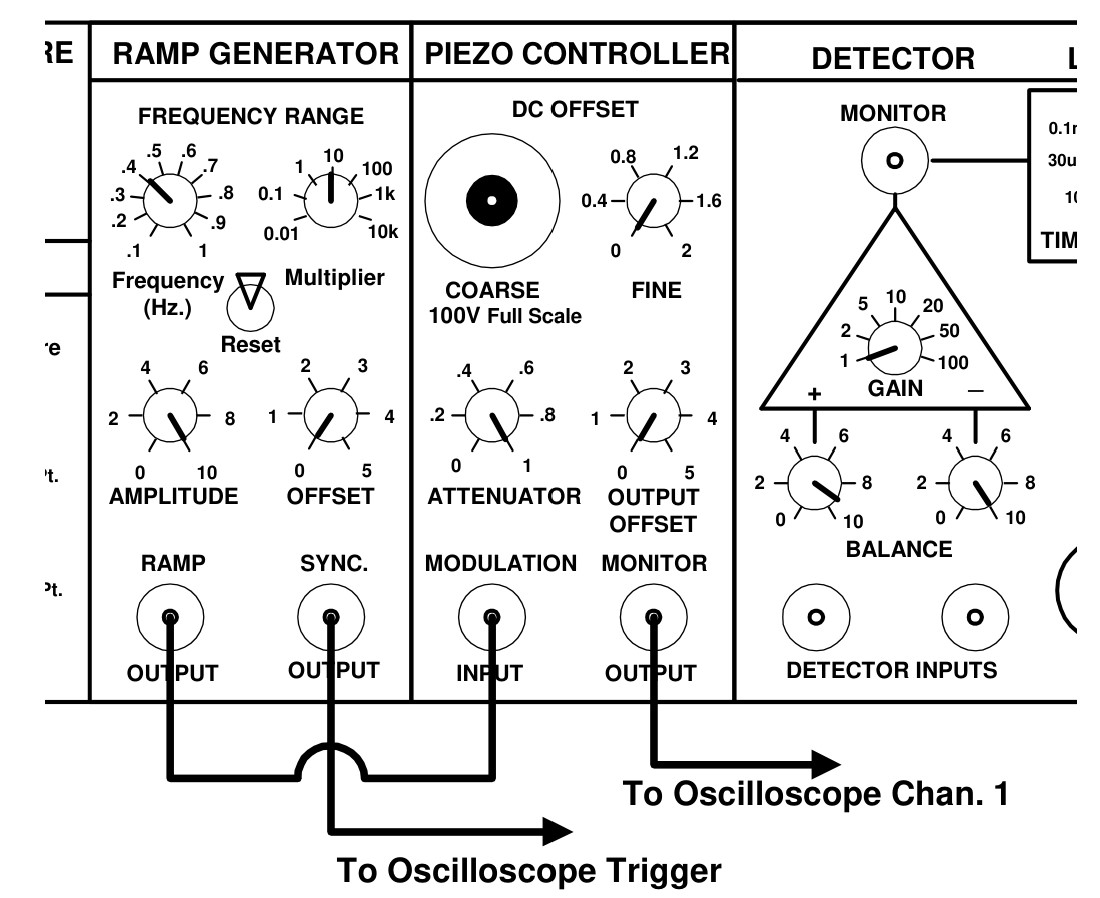
\includegraphics[width=0.5\textwidth]{content/graphics/controller.jpg}
    \caption{Series of pictures of the external and internal cavity modes as the grating angle decreased.\cite{diode_laser}} %\cite
    \label{fig:contr} 
\end{figure}
To record different resonance and fluorescence lines of rubidium an oscilloscope is connected. 
A camera connected to a TV is available to take pictures of the fluorescence and the light from the laser
